\documentclass[english]{scrartcl}
\usepackage[T1]{fontenc}
\usepackage[latin9]{inputenc}
\usepackage{babel}
\usepackage{graphicx}
\usepackage{listings}
\usepackage{amsmath}
\usepackage{url}
% 
\renewcommand{\tt}{\normalfont \ttfamily}

\begin{document}
\title{Fitting ALS Reflectance Data using Python, Version 1.0}
\author{R. Steven Turley}
\date{April, 2018}

\maketitle
\tableofcontents{}

\section{Introduction}

This report explains how to use Python to fit reflectance data
taken in Beamline 6.3.2 at the Advanced Light Source at Lawrence
Berkeley National Lab. It is based on some classes I wrote to
make the processes somewhat easier.

\subsection{Python}
If you don't already know at least a little Python, I would suggest
reading a python tutorial before reading this. I'll explain
things a little bit along the way, but the purpose of this document
is more about fitting the data than about learning Python.

\subsection{Fitting Steps}
There are a couple of steps to the fitting process:
\begin{itemize}
\item reading in raw data
\item combining raw data files to compute $\theta$/$2\theta$ spectra
\item fitting the $\theta$/$2\theta$ spectra to theoretical curves
\item combining the fits to derive average data values
\item refitting the data with average data values.
\end{itemize}

\subsection{Refl Module}
The library routines and classes you'll need to do the fitting
are in the file \texttt{refl.py}. Before using these routines and
classes, you'll need to import with the entire module
\begin{lstlisting}
import refl
\end{lstlisting}
or the specific items you need from the module.
\begin{lstlisting}
from refl import Spectrum, Index, Parratt
\end{lstlisting}
The \texttt{refl} module contains the following items.
\begin{description}
\item [matR] a function to calculate reflectance and transmittance
	from a multilayer mirror using matrices. It is slower than
	Parratt if you only want the reflectance.
\item [Parratt] a function to calculated reflectance from a
	multilayer mirror.
\item [fracs] a function to calculate the fraction of s-polarized
	light in the synchrotron beam at the ALS. This is mostly used
	internally.
\item [Index] a class returning the complex index of refraction
	for a material.
\item [Run] a class with the raw data from a run.
\item [Runs] a cache of all of the run data form an ALS
	trip. Runs[i] is the Run numbered i.
\item [Reflectance] a class with computed reflectance from a set
	of runs.
\item [Log] a class with information from the log file saved
	with a set of runs.
\end{description}

\section{Reading Raw Data Files}
Raw data files from the ALS consists of a header line with data
information followed by four columns of numbers:
\begin{description}
\item [var] the data being varied during the measurement. For
	$\theta$/$2\theta$ measurements (our most common ones), this
	is the measurement angle. For $I_0$ measurements, this is the
	wavelength. For dark current measurements, this is usually
	the time.
\item [diode] the signal from the diode detector
\item [m3] the signal from the m3 mirror (usually ignored)
\item [beam] the beam current during the run (also usually ignored)
\end{description}
There are three classes in \texttt{refl} which manage these data files
for you.
\subsection{Log class}
The Log class parses the log file with information about each run. The command
\begin{lstlisting}
log = Log('../ALSdata','Feb2018')
\end{lstlisting}
will read the log file in the directory \texttt{../ALSdata} with the
name \texttt{Feb2018.log} and store it as the log object. There are various
attributes stores as arrays in object.
\begin{description}
\item[filename] the filename for the run
\item[fullname] the complete filename with path for the run
\item[comment] the comment stored with the run
\item[date] the date of the run
\item[time] the time of the run
\item[gain] the log (base 10) of the gain for this run
\item[wavelength] the wavelength in nm (usually) for this run
\end{description}
Some of this information is copied to Run objects when they are created.
\subsection{Run class}
A Run object has the raw data for a single run. It is usually accessed
from the Runs class rather than directly. This permits read caching. It has the
four attributes mentioned above for each run (stored as np.array objects) as well
as the wavelength, comment, and gain from the log file.
The Run class has a plot method defined which will plot the data for a run
using the comment as the plot title. Figure~\ref{fig:run102} was generated
using the following command.
\begin{lstlisting}
runs[102].plot()
\end{lstlisting}
\begin{figure}[htb]
  \begin{center}
    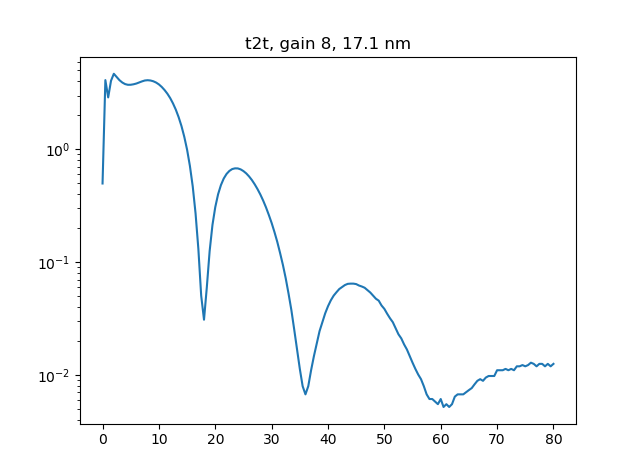
\includegraphics[width=0.75\textwidth]{images/run102}
  \end{center}
  \caption{\label{fig:run102}raw data from run 102}
\end{figure}

\subsection{Runs class}
The Run objects are returned by the Runs class which reads the files
when needed and caches their contents for subsequent calls. After executing
\begin{lstlisting}
runs = Runs(log)
\end{lstlisting}
the individual run information can be accessed as \texttt{runs[rnum]} where
rnum is the run number. Thus, the gain for run 11 would be \texttt{runs[11].gain}.

\section{Creating Reflectance Spectra}
Reflectance spectra are created with with the Reflectance class by combining
various runs to find $I$, $I_0$, and associated gains, and the associated
dark currents.

I will illustrate how this is done by creating two single spectra and them combining
and filtering them. I've used the data taken on Feb 24, 2018 at the
Advanced Light Source for sample 180221A at 18~nm as the example.

\subsection{Creating a Single Spectrum}

The first step is to import the libraries needed for the analysis. We will
refl for this library, numpy for finding the mean of arrays, matplotlib
to plot the results, and scipy for the fitting routine.
\begin{lstlisting}
import refl
import numpy as np
import matplotlib.pyplot as plt
from scipy.optimize import curve_fit
\end{lstlisting}
Next we need to create a Log and Runs objects with the data from the run.
\begin{lstlisting}
log = refl.Log('../ALSdata','Feb2018')
runs = refl.Runs(log)
\end{lstlisting}
The next step is to create a tuple of dark currents from the run. The dark
currents were in runs 101 (gain 7), 98 (gain 8), 99 (gain 9), and 100 (gain 10).
The dark current is computed as the mean diode signal for a dark current run.
\begin{lstlisting}
d7=np.mean(runs[101].diode)
d8=np.mean(runs[98].diode)
d9=np.mean(runs[99].diode)
d10=np.mean(runs[100].diode)
dark=(d7,d8,d9,d10)
\end{lstlisting}

There were three runs with $\theta$/$2\theta$ data for this sample at 18~nm.
Run 119 was taken with a lower gain than runs 120 and 121. Runs 120 and 121
don't have any data for the lowest angles.
I'll create separate spectra for these two sets of runs
to make it easier to filter and combine them. The $I0$ data for this filter and
sample is in run 97.
\begin{lstlisting}
s18a = refl.Reflectance((runs[119],),runs[97], dark)
plt.figure()
plt.semilogy(s18a.ang, s18a.rfl)
plt.title('Spectrum 18a')
s18b = refl.Reflectance((runs[120], runs[121]), runs[97], dark)
plt.figure()
plt.semilogy(s18b.ang, s18b.rfl)
plt.title('Spectrum 18b')
\end{lstlisting}
The plot commands in the above listing produced the plots in
Figures~\ref{fig:18a} and \ref{fig:18b}
\begin{figure}[htb]
  \begin{center}
    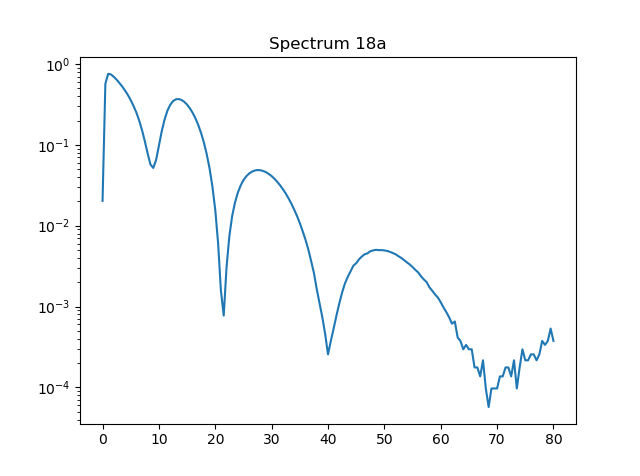
\includegraphics[width=0.75\textwidth]{images/r18a}
  \end{center}
  \caption{\label{fig:18a}reflectance data from run 119}
\end{figure}
\begin{figure}[htb]
  \begin{center}
    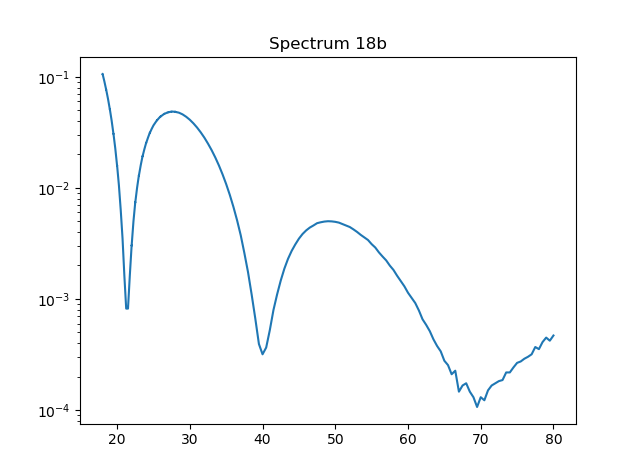
\includegraphics[width=0.75\textwidth]{images/r18b}
  \end{center}
  \caption{\label{fig:18b}reflectance data from combining runs 120 and 121}
\end{figure}

\subsection{Combining Spectra}
By looking at the the raw data, I
decided that the best data for angles of $18^\circ$ or less is run 119 and the best
data for angles greater than $18^\circ$ is the combination of runs 120 and 121.
To combine the runs, I filtered spectrum s18a to only have angles up to $18^\circ$.
I also eliminated the angles less than two degrees where it is unreliable. I
filtered the spectrum 18b to only include the data for angles greater than
$18^\circ$. I then added the two spectra together to get a combined spectrum s18
which is shown in Figure~\ref{fig:18}
\begin{lstlisting}
s18 = s18a.filter(2,18) + s18b.filter(18.05,80)
s18.plot()
\end{lstlisting}
\begin{figure}[htb]
  \begin{center}
    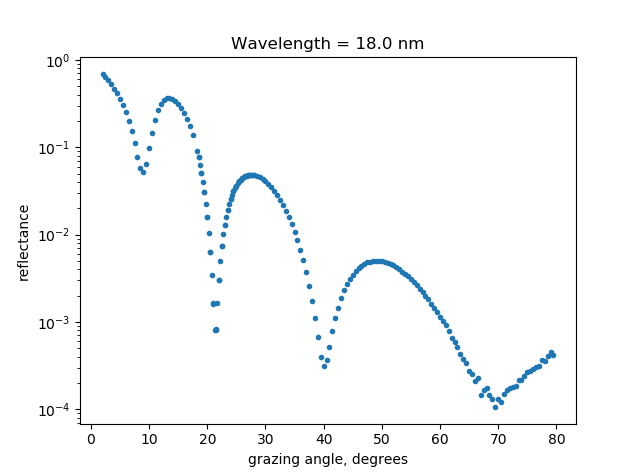
\includegraphics[width=0.75\textwidth]{images/r18}
  \end{center}
  \caption{\label{fig:18}reflectance data from combining runs 120 and 121}
\end{figure}

\section{Fitting the Data}
Once we have the reflectance spectrum, we need to find the materials properties
that provide the best match between our reflectance measurements and theoretical
calculations. We call this process data fitting.

\subsection{Mirror Model}
Based on our fabrication process and the measurements we made prior to
going to ALS, we think this sample has a thick Si$_3$N$_4$ substrate followed
by a layer of Al and AlF$_3$.We are not sure about the thickness of the Al or
AlF$_3$ layers, but we think the have respective thicknesses of 8~nm and 26~nm. To
start with we will assume the Al is unoxidized and has a complex index of
refraction given by the data file in volta.

The refl library has two routines for computing reflectance, \texttt{Parratt}
and \texttt{matR}. We'll use \texttt{Parratt} for this example since we only
care about reflectance and now about transmittance in this case. The \texttt{Parratt}
function takes the following arguments.
\begin{description}
\item[n] a numpy array with the index of refraction of the various layers. It starts
with the index of refraction of the incident layer (which is a vacuum in our case)
and works its way down to the substrate.
\item{x} a numpy array with the thicknesses of each mirror layer in
nanometers. The thickness of
the incident (vacuum) layer and substrate layers should be set to 0. This is because we
are interested in the field right at the interface; not after is has penetrated into those
layers.
\item[thetad] the incident angle measured from grazing in degrees
\item[lam] the wavelength in nanometers
\item[frs] the fraction of s polarization in the beam. If left to its default
value of 0, the Gullikson formula is used.
\item[sigma] an array or tuple
with the rms roughness of each interface measured in nm. They
should be in the same order as the layers themselves. There is one less interface than
layers, so this array will be one smaller than the n and x arrays.
\end{description}
\subsection{Index of Refraction}
We will look up the index of refraction (either as starting guesses or assumed
exact values) from tables we store on the volta server. The Index class in refl
will read these values in these tables from volta. They have an at function
which interpolates between the values in these tables to estimate the index
of refraction at our desired wavelength.  This code creates Index objects
for AlF$_3$, Al, and Si$_3$N$_4$.
\begin{lstlisting}
# index objects
AlF3Index = refl.Index("AlF3")
AlIndex = refl.Index("Al")
Si3N4Index = refl.Index("Si3N4")
# interpolated values at 18 nm
alf3ndx = AlF3Index.at(s18.wavelength)
alndx = AlIndex.at(s18.wavelength)
si3n4ndx = Si3N4Index.at(s18.wavelength)
\end{lstlisting}
\subsection{Create Fit Function}
The \texttt{curve\_fit} function will call a function we need to write to
compute the theoretical reflectance using the current value of the parameters
it is trying to fit. The function will have the desired angles as its first
argument and successive parameters values as subsequent arguments.  Our
parameters for this first fit
will be the read and imaginary parts of the AlF$_3$ index of refraction (n and k),
the thickness of the AlF$_3$ layer (tf), and the thickness of the Al layer (ta).
\begin{lstlisting}
def f(thr, n, k, tf, ta):
    ndx = np.array([1+0j, n+k*1j, alndx, si3n4ndx])
    th = np.array([0, tf, ta, 0])
    sigma = (1.0,0,0);
    return [refl.Parratt(ndx ,th, thetad, s18.wavelength, 0, 
    	sigma) for thetad in thr]
\end{lstlisting}
The function uses the passed parameters to set up the index of refraction
array and the thickness array for the call to \texttt{Parratt}. \texttt{Parratt}
is then called to compute the reflectance with these parameters at the passed
values for theta.
If we want to fit different parameters, we'll have to edit this function because
its calling arguments will change.

\subsection{Weights}
Because of the wide range of values covered by the reflectance and
the obvious noise floor at the highest angles, it is important to
use a weighted fit. The challenge, which involves as much art as
science, is to choose a reasonable set of weights. Based on experience
and other studies, I'm inclined to use a weight with two components
in quadrature. The first will be an exponentially decreasing function
whose log has the same slope as the average log of the slope of the
data. The second term will be a constant value with a magnitude of the
lowest data points.
\begin{eqnarray}
\sigma_i &=& \sqrt{\sigma_p^2+\sigma_c^2}\\
\sigma_p &=& \alpha \exp(-\beta\theta_i)\\
\sigma_c &=& \gamma
\end{eqnarray}
I'll start with $\alpha=0.05$, $\beta=0.097$,
and $\gamma=5\times 10^{-5}$. I chose $\alpha$ of this size because a
5\% error seems like a good starting guess. $\beta$ was chosen by
eyeballing the slope of the data in Figure~\ref{fig:18} and estimating
the average slope of the data. $\gamma$ was chosen by estimating the size
of the noise around the lowest data points near $70^\circ$. Here is
the Python code to implement this.
\begin{lstlisting}
alpha = 0.2
beta = 0.097
gamma = 5e-5
sigmap = np.array([alpha*np.exp(-beta*th) for th in s18.ang])
sigmac = gamma
sigmaw = np.sqrt(sigmap**2+sigmac**2)
\end{lstlisting}

\subsection{Fit}
The last thing we need for the fit are starting guesses for
the fir parameters.I used approximated values of $n$ and $k$
from the table values in volta. This thickness estimates came from
information supplied by David Allred from ellipsometry data. These
are stored in the array \texttt{p0}.
\begin{lstlisting}
p0=np.array([0.95, 0.025, 8, 26])
\end{lstlisting}
Finally, the \texttt{curve\_fit} routine is called using the above
parameters.
\begin{lstlisting}
popt, pcov = curve_fit(f, s18.ang, s18.rfl, p0, sigmaw,
                       absolute_sigma=False)
\end{lstlisting}
It has the following arguments:
\begin{description}
\item[f] the function to compute the reflectance given the parameters
\item[s18.ang] the angles at which the reflectance was measured
\item[s18.rfl] the measured reflectance
\item[p0] the initial values of the fit parameters
\item[sigmaw] the weight for each point
\item[absolute\_sigma] whether the weight should be considered as the
\item[popt] returned value of the optimum parameters
\item[pcov] returned value of the estimated covariance matrix
absolute uncertainty or a relative value. For this initial fit where I do
not yet know the residual, using a relative value makes sense.
\end{description}
Figure~\ref{fig:fit18} shows the results of this fit and the value of
\texttt{sigmaw} I used.
\begin{figure}[htb]
  \begin{center}
    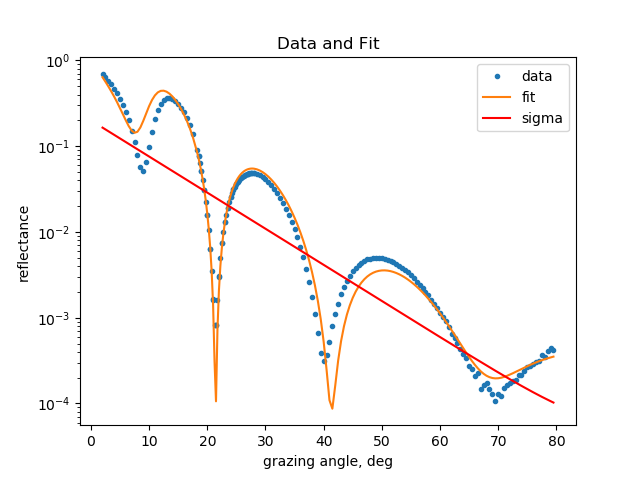
\includegraphics[width=0.75\textwidth]{images/fit18}
  \end{center}
  \caption{\label{fig:fit18}data, initial fit, and weights for
  sample 180221A at 18~nm}
\end{figure}
The elements of \texttt{popt} are the returned valued of the
optimal fit parameters. The diagonal elements of the covariance matrix
in pcov give the estimated uncertainty in these parameters. This
code will print those values.
\begin{lstlisting}
print('n = '+str(round(popt[0],4))+"+/-"+
      str(round(np.sqrt(pcov[0,0]),4)))
print('k = '+str(round(popt[1],4))+"+/-"+
      str(round(np.sqrt(pcov[1,1]),2)))
print('tf = '+str(round(popt[2],2))+"+/-"+
      str(round(np.sqrt(pcov[2,2]),2)))
print('ta = '+str(round(popt[3],4))+"+/-"+
      str(round(np.sqrt(pcov[3,3]),2)))
\end{lstlisting}
This returns the following:
\begin{lstlisting}
n = 0.9784+/-0.0011
l = 0.0301+/-0.0
tf = 8.93+/-0.1
ta = 24.5396+/-0.21
\end{lstlisting}
These are close to our original parameter guesses and have reasonable
uncertainties.
The code use to create the plot in Figure~\ref{fig:fit18} is as follows.
\begin{lstlisting}
rfit = f(s18.ang, popt[0], popt[1], popt[2], popt[3])
plt.figure()
plt.semilogy(s18.ang, s18.rfl,'.',s18.ang, rfit, '-',
	s18.ang, sigmaw,'-r')
plt.title('Data and Fit')
plt.xlabel('grazing angle, deg')
plt.ylabel('reflectance')
plt.legend(['data', 'fit','sigma'])
\end{lstlisting}
The function \texttt{f} was called to compute the fit function using the optimal parameter values returned by \texttt{curve\_fit}.
\subsection{Discussion of Results}
The fit shows there are some obvious problems with the model we used
for our data. There is a relatively large difference between the depth of
the first minimum near $10^circ$. This is probably more than just an alignment
error. Secondly, the minimum values in the measured data are not as deep
as calculated by the model. For valleys which are this deep and with such
large slopes, this can be due variations in thin film thickness over the
size of the beam spot and the angular spread in the incident beam.
Finally, the location of the interference minima don't match the data
very well. This is probably an artifact of our chosen weights and an
error in the rest of the model. To understand the artifact in the weight,
not that the weight at $20^\circ$ is about 300 times larger than the
fit minimum at that point. With our 5\% guess in the uncertainty, this
is well within the bounds of what we'd expect. We can force a better fit
of these minima by having the weights be proportional to the 
measured data. Here is the code for a refit with those weights.
\begin{lstlisting}
sigmap = alpha*np.abs(s18.rfl)
sigmaw = np.sqrt(sigmap**2+sigmac**2)
popt, pcov = curve_fit(f, s18.ang, s18.rfl, p0, sigmaw,
                       absolute_sigma=False)
\end{lstlisting}
The fit is shown in Figure~\ref{fig:fit18a}.
\begin{figure}[htb]
  \begin{center}
    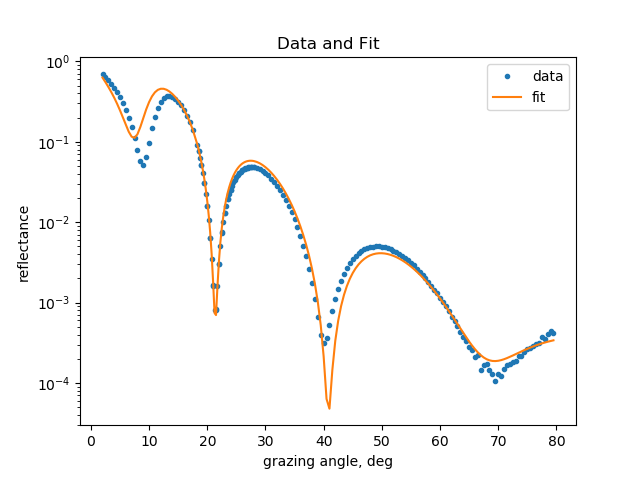
\includegraphics[width=0.75\textwidth]{images/fit18a}
  \end{center}
  \caption{\label{fig:fit18a}refit for sample 180221A at 18~nm using
  weights proportional to the data}
\end{figure}
The optimal fir parameters were
\begin{lstlisting}
n = 0.9768+/-0.0011
k = 0.0249+/-0.0
tf = 8.67+/-0.1
ta = 25.3344+/-0.15
\end{lstlisting}
Not that forcing a better fit to the valleys brings the imaginary
part of the AlF$_3$ index of refraction closer to the tabulated
values.

We can check the value of $\beta$ we chose by calculating
\begin{equation}
\chi^2=\sum_i\left(\frac{f_i-y_i}{\sigma_i}\right)^2\;.
\end{equation}
This should be approximately equal to the number of data points
if $\beta$ was chosen correctly (at least if the errors were statistical).
With this code
\begin{lstlisting}
chi2 = np.sum(((s18.rfl-rfit)/sigmaw)**2)
print('chi**2 = '+str(round(chi2,1))+" npts = "+
	str(np.size(sigmaw)))
\end{lstlisting}
I get $\chi^2=941.7$ with 195 data points. This says an 11\% error
would have been a better guess of $\beta$ than the 5\% value
I used.
\subsection{Improved Model}
It's probable that the Al was at least partially oxidized. We could
put this in out model as the addition of an Al$_2$O$_3$ layer on top
of the Al, or as an altered effective index of refraction for the
Al. Let's try both and see which improves the fit the most. First we'll
try fitting adding additional oxide layer.
The following code allows us to add an oxide layer and fit its
thickness.
\begin{lstlisting}
Al2O3Index = refl.Index("Al2O3")
al2o3ndx = Al2O3Index.at(s18.wavelength)
def f2(thr, n, k, tf, ta, to):
    ndx = np.array([1+0j, n+k*1j, al2o3ndx, alndx, si3n4ndx])
    th = np.array([0, tf, to, ta, 0])
    sigma = np.array([1.0,0,0,0]);
    return [refl.Parratt(ndx ,th, thetad, s18.wavelength, 0, sigma)
            for thetad in thr]
p0=np.array([0.95, 0.025, 8, 26, 1])
popt, pcov = curve_fit(f2, s18.ang, s18.rfl, p0, sigmaw,
                       absolute_sigma=False)
\end{lstlisting}
The fit indeed improves, as shown in Figure~\ref{fig:fit18oxide}, but
does so by requiring an unphysical value for the fluoride thickness.
\begin{lstlisting}
n = 1.3424+/-0.0291
k = 0.1928+/-0.02
tf = 0.19+/-0.03
ta = 26.3502+/-0.14
to = 5.4362+/-0.0802
\end{lstlisting}
\begin{figure}[htb]
  \begin{center}
    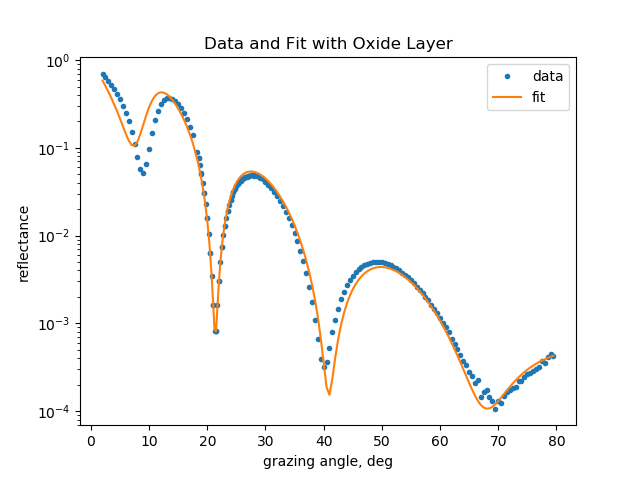
\includegraphics[width=0.75\textwidth]{images/fit18oxide}
  \end{center}
  \caption{\label{fig:fit18oxide}fit for sample 180221A at 18~nm using
  an Al$_2$O$_3$ layer}
\end{figure}
For this approach to work, we should find average values of the
layer thickness as described in Section~\ref{sec:avg} and then refit
using these average values as described in Section~\ref{sec:refit}.

Let's see what happens if we allow the index of refraction of the Al
layer to change rather than adding an oxide layer. Here is the code for
that.
\begin{lstlisting}
def f3(thr, nf, kf, na, ka, tf, ta):
    ndx = np.array([1+0j, nf+kf*1j, na+ka*1j, si3n4ndx])
    th = np.array([0, tf, ta, 0])
    sigma = np.array([1.0,0,0]);
    return [refl.Parratt(ndx ,th, thetad, s18.wavelength, 0, sigma)
            for thetad in thr]
p0=np.array([0.95, 0.025, alndx.real, alndx.imag, 8, 26])
popt, pcov = curve_fit(f3, s18.ang, s18.rfl, p0, sigmaw,
                       absolute_sigma=False)
\end{lstlisting}
As shown in Figure~\ref{fig:fit18alndx}, this improves the fit a lot
for the low angles, although the fit at the highest angles is still
problematic. Here are the fit values.
\begin{lstlisting}
nf = 0.9809+/-0.0008
kf = 0.036+/-0.0008
na = 1.0019+/-0.0004
ka = 0.0011+/-0.0004
tf = 8.82+/-0.0675
ta = 25.2063+/-0.1068
\end{lstlisting}
The fit constants are physically reasonable when we note that the
index of refraction of Al at 18~nm is $1.0087+0.0024i$.
\begin{figure}[htb]
  \begin{center}
    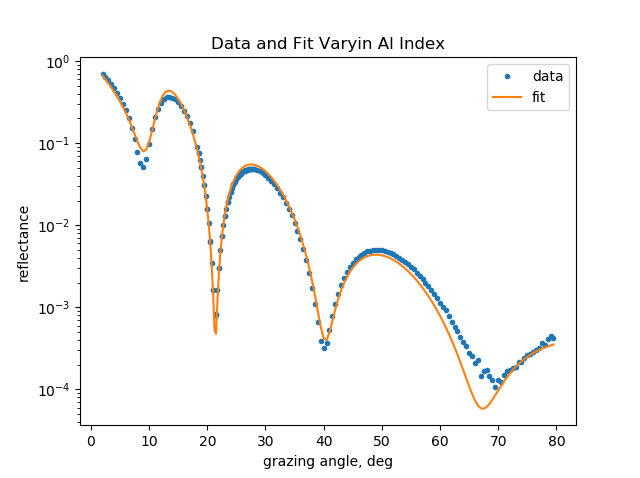
\includegraphics[width=0.75\textwidth]{images/fit18alndx}
  \end{center}
  \caption{\label{fig:fit18alndx}fit for sample 180221A at 18~nm using
  an Al$_2$O$_3$ layer}
\end{figure}
The best model of the mirror in the end will probably use a fitted value
for the Al index of refraction to compensate for the fact that
our Al probably isn't perfect and a thin oxide layer as well.

\section{Finding Average Values}\label{sec:avg}
The thickness of the mirror films should change with wavelength, the the
index of refraction of the mirror layers will. The best overall strategy
for fitting the data would be to fit the thickness at multiple wavelengths
and then use an average thickness as characteristic for all layers.
then we should go back and refit the data keeping the thicknesses
constant (or maybe only varying the thickness of the Al2O3 layer).
By thus iterating, we should get a better physical model.

I'll complete this section after a student goes through and actually
does these fits as suggested for the rest of the wavelengths we measured.

\section{Refitting Data}\label{sec:refit}
This section will have the results of the final fits when we've only
fit the index of refraction and kept the layer thicknesses the same
for all samples.

\appendix
\section{Complete Python Code}
This is the complete python code I used for the analysis described here.
\begin{lstlisting}
# -*- coding: utf-8 -*-
"""
Created on Thu Apr 26 11:50:40 2018

@author: rturley
"""

import refl
import numpy as np
import matplotlib.pyplot as plt
from scipy.optimize import curve_fit


# log = refl.Log('../ALSdata','Feb2018') # NSF computer
log = refl.Log() # BYU Computer
runs = refl.Runs(log)

# dark current calculation
d7=np.mean(runs[101].diode)
d8=np.mean(runs[98].diode)
d9=np.mean(runs[99].diode)
d10=np.mean(runs[100].diode)
dark=(d7,d8,d9,d10)

# runs
s18a = refl.Reflectance((runs[119],),runs[97], dark)
plt.figure()
plt.semilogy(s18a.ang, s18a.rfl)
plt.title('Spectrum 18a')
s18b = refl.Reflectance((runs[120], runs[121]), runs[97], dark)
plt.figure()
plt.semilogy(s18b.ang, s18b.rfl)
plt.title('Spectrum 18b')

s18 = s18a.filter(2,18) + s18b.filter(18.05,80)
s18.plot()

# index objects
AlF3Index = refl.Index("AlF3")
AlIndex = refl.Index("Al")
Si3N4Index = refl.Index("Si3N4")
# interpolated values at 18 nm
alf3ndx = AlF3Index.at(s18.wavelength)
alndx = AlIndex.at(s18.wavelength)
si3n4ndx = Si3N4Index.at(s18.wavelength)

# fit function
def f(thr, n, k, tf, ta):
    ndx = np.array([1+0j, n+k*1j, alndx, si3n4ndx])
    th = np.array([0, tf, ta, 0])
    sigma = np.array([1.0,0,0]);
    return [refl.Parratt(ndx ,th, thetad, s18.wavelength, 0, sigma)
            for thetad in thr]

alpha = 0.2
beta = 0.097
gamma = 5e-5
sigmap = np.array([alpha*np.exp(-beta*th) for th in s18.ang])
sigmac = gamma
sigmaw = np.sqrt(sigmap**2+sigmac**2)
p0=np.array([0.95, 0.025, 8, 26])
popt, pcov = curve_fit(f, s18.ang, s18.rfl, p0, sigmaw,
                       absolute_sigma=False)
print('n = '+str(round(popt[0],4))+"+/-"+
      str(round(np.sqrt(pcov[0,0]),4)))
print('k = '+str(round(popt[1],4))+"+/-"+
      str(round(np.sqrt(pcov[1,1]),2)))
print('tf = '+str(round(popt[2],2))+"+/-"+
      str(round(np.sqrt(pcov[2,2]),2)))
print('ta = '+str(round(popt[3],4))+"+/-"+
      str(round(np.sqrt(pcov[3,3]),2)))
rfit = f(s18.ang, popt[0], popt[1], popt[2], popt[3])
plt.figure()
plt.semilogy(s18.ang, s18.rfl,'.',s18.ang, rfit, '-',
             s18.ang, sigmaw,'-r')
plt.title('Data and Fit')
plt.xlabel('grazing angle, deg')
plt.ylabel('reflectance')
plt.legend(['data', 'fit','sigma'])

# refit with weights proportional to the data
sigmap = alpha*np.abs(s18.rfl)
sigmaw = np.sqrt(sigmap**2+sigmac**2)
popt, pcov = curve_fit(f, s18.ang, s18.rfl, p0, sigmaw,
                       absolute_sigma=False)
print('n = '+str(round(popt[0],4))+"+/-"+
      str(round(np.sqrt(pcov[0,0]),4)))
print('k = '+str(round(popt[1],4))+"+/-"+
      str(round(np.sqrt(pcov[1,1]),2)))
print('tf = '+str(round(popt[2],2))+"+/-"+
      str(round(np.sqrt(pcov[2,2]),2)))
print('ta = '+str(round(popt[3],4))+"+/-"+
      str(round(np.sqrt(pcov[3,3]),2)))
rfit = f(s18.ang, popt[0], popt[1], popt[2], popt[3])
plt.figure()
plt.semilogy(s18.ang, s18.rfl,'.',s18.ang, rfit, '-')
plt.title('Data and Fit')
plt.xlabel('grazing angle, deg')
plt.ylabel('reflectance')
plt.legend(['data', 'fit'])

# Check \chi^2
chi2 = np.sum(((s18.rfl-rfit)/sigmaw)**2)
print('chi**2 = '+str(round(chi2,1))+" npts = "+
      str(np.size(sigmaw)))

# Add Al2O3 layer
Al2O3Index = refl.Index("Al2O3")
al2o3ndx = Al2O3Index.at(s18.wavelength)
def f2(thr, n, k, tf, ta, to):
    ndx = np.array([1+0j, n+k*1j, al2o3ndx, alndx, si3n4ndx])
    th = np.array([0, tf, to, ta, 0])
    sigma = np.array([1.0,0,0,0]);
    return [refl.Parratt(ndx ,th, thetad, s18.wavelength,
            0, sigma) for thetad in thr]
p0=np.array([0.95, 0.025, 8, 26, 1])
popt, pcov = curve_fit(f2, s18.ang, s18.rfl, p0, sigmaw,
                       absolute_sigma=False)
print('n = '+str(round(popt[0],4))+"+/-"+
      str(round(np.sqrt(pcov[0,0]),4)))
print('k = '+str(round(popt[1],4))+"+/-"+
      str(round(np.sqrt(pcov[1,1]),2)))
print('tf = '+str(round(popt[2],2))+"+/-"+
      str(round(np.sqrt(pcov[2,2]),2)))
print('ta = '+str(round(popt[3],4))+"+/-"+
      str(round(np.sqrt(pcov[3,3]),2)))
print('to = '+str(round(popt[4],4))+"+/-"+
      str(round(np.sqrt(pcov[4,4]),4)))
rfit = f2(s18.ang, popt[0], popt[1], popt[2], popt[3], popt[4])
plt.figure()
plt.semilogy(s18.ang, s18.rfl,'.',s18.ang, rfit, '-')
plt.title('Data and Fit with Oxide Layer')
plt.xlabel('grazing angle, deg')
plt.ylabel('reflectance')
plt.legend(['data', 'fit','sigma'])

# Fit Al index of refraction
def f3(thr, nf, kf, na, ka, tf, ta):
    ndx = np.array([1+0j, nf+kf*1j, na+ka*1j, si3n4ndx])
    th = np.array([0, tf, ta, 0])
    sigma = np.array([1.0,0,0]);
    return [refl.Parratt(ndx ,th, thetad, s18.wavelength,
    		0, sigma) for thetad in thr]
p0=np.array([0.95, 0.025, alndx.real, alndx.imag, 8, 26])
popt, pcov = curve_fit(f3, s18.ang, s18.rfl, p0, sigmaw,
                       absolute_sigma=False)
print('nf = '+str(round(popt[0],4))+"+/-"+
      str(round(np.sqrt(pcov[0,0]),4)))
print('kf = '+str(round(popt[1],4))+"+/-"+
      str(round(np.sqrt(pcov[1,1]),4)))
print('na = '+str(round(popt[2],4))+"+/-"+
      str(round(np.sqrt(pcov[2,2]),4)))
print('ka = '+str(round(popt[3],4))+"+/-"+
      str(round(np.sqrt(pcov[3,3]),4)))
print('tf = '+str(round(popt[4],4))+"+/-"+
      str(round(np.sqrt(pcov[4,4]),4)))
print('ta = '+str(round(popt[5],4))+"+/-"+
      str(round(np.sqrt(pcov[5,5]),4)))
rfit = f3(s18.ang, popt[0], popt[1], popt[2], popt[3],
	      popt[4], popt[5])
plt.figure()
plt.semilogy(s18.ang, s18.rfl,'.',s18.ang, rfit, '-')
plt.title('Data and Fit Varyin Al Index')
plt.xlabel('grazing angle, deg')
plt.ylabel('reflectance')
plt.legend(['data', 'fit','sigma'])
\end{lstlisting}

\end{document}